\section{Hardware}
En la figura \ref{fig:circuito} se muestra el diagrama a bloques del módulo de monitoreo que será utilizado para realizar la medición de la potencia activa que proviene del sistema fotovoltaico. \\
Se puede observar la entrada a nuestro sistema, la cual está dada por el voltaje y la corriente producida por la fuente de energía fotovoltaica; la comunicación que existirá entre el monitor de potencia con el microcontrolador, así como la comunicación entre el microcontrolador y el módulo WiFi; este último módulo a su vez estará comunicándose con el servidor embebido por medio del protocolo TCP.  
\\
\begin{figure}[H]
	\centering
	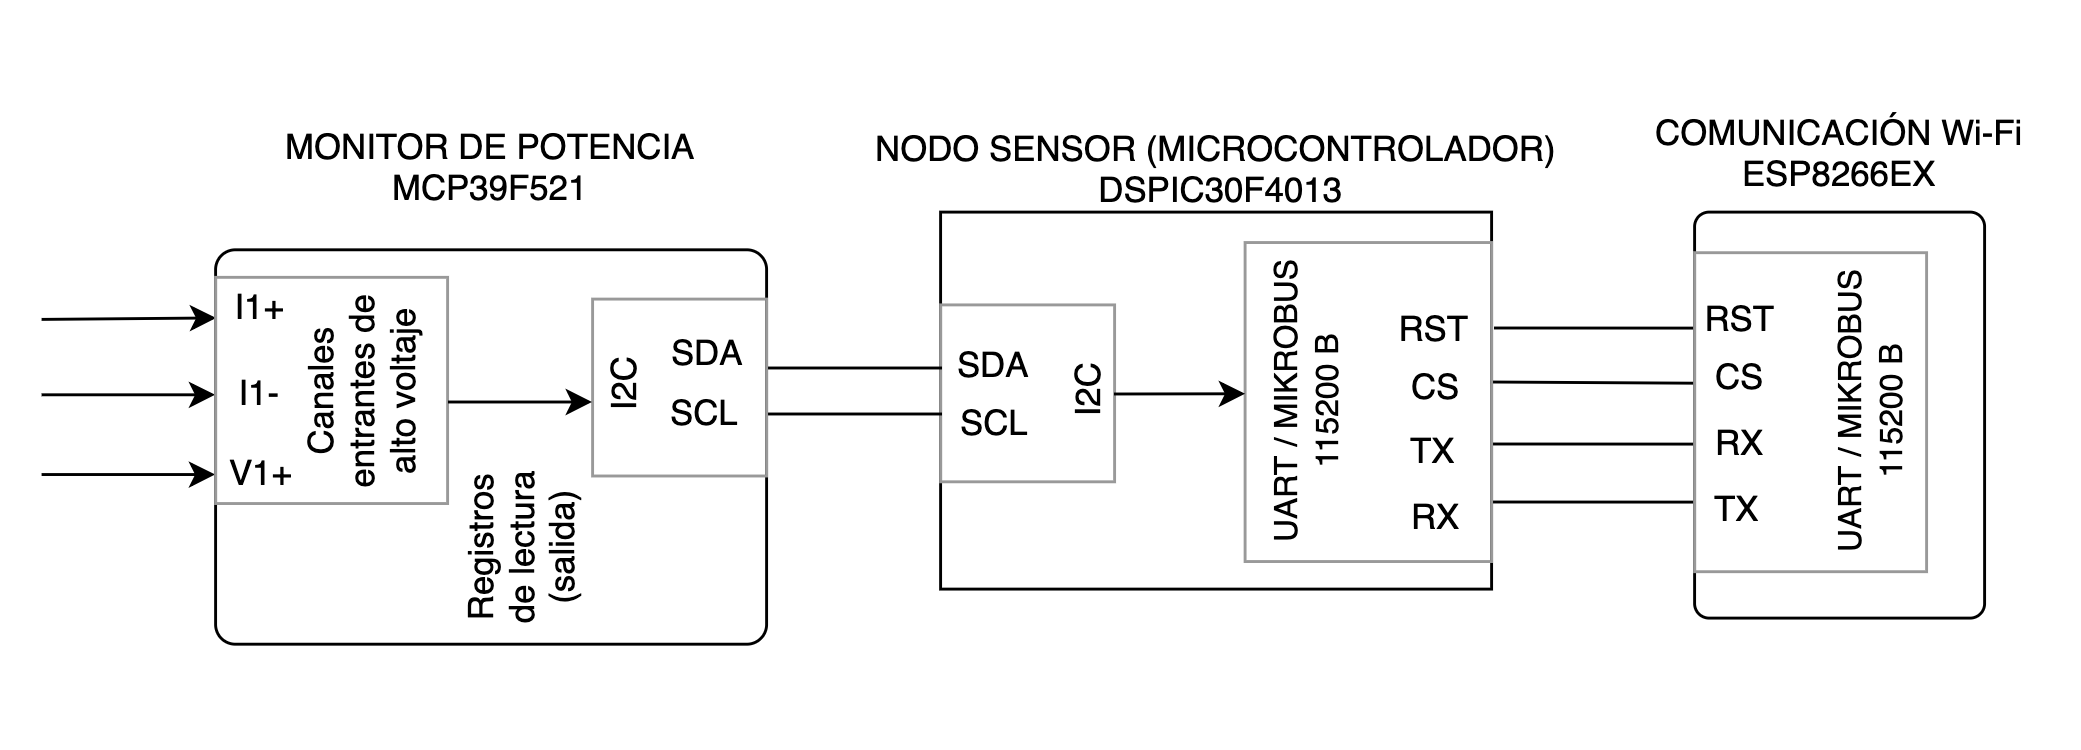
\includegraphics[width=1\textwidth]{Capitulo4/hardware/images/sistemaDigital.png}
	\caption{Diagrama a bloques del módulo de monitoreo}
	\label{fig:circuito}
\end{figure}

%%\subsection{Submódulo Mediciones}
En la imagen \ref{fig:CircuitoCau} se muestra la conexión correspondiente al caudalimetro.

\begin{figure}[H]
	\centering
	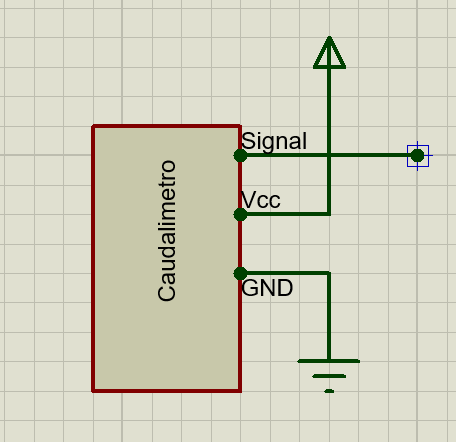
\includegraphics[width=0.5\textwidth]{Capitulo4/hardware/images/CircuitoCaudalimetro}
	\caption{Circuito del sensor}
	\label{fig:CircuitoCau}
\end{figure}
%\subsection{Submódulo Microcontrolador}
En la imagen \ref{fig:CircuitoMicro} se muestra la conexión correspondiente al microcontrolador.

\begin{figure}[H]
	\centering
	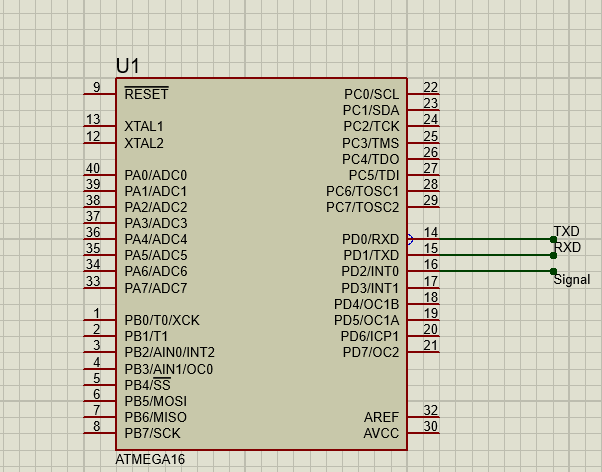
\includegraphics[width=0.5\textwidth]{Capitulo4/hardware/images/CircuitoMicrocontrolador}
	\caption{Circuito del microcontrolador}
	\label{fig:CircuitoMicro}
\end{figure}
%\subsection{Submódulo Comunicación inalámbrica}
En la imagen \ref{fig:CircuitoBlue} se muestra la conexión correspondiente al módulo bluetooth HC-05.

\begin{figure}[H]
	\centering
	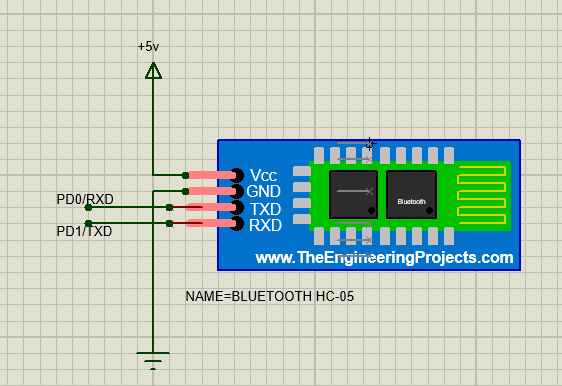
\includegraphics[width=0.5\textwidth]{Capitulo4/hardware/images/CircuitoBluetooth}
	\caption{Circuito del módulo bluetooth}
	\label{fig:CircuitoBlue}
\end{figure}